%%%%%%%%%%%%%%%%%%%%%%%%%%%%%%%%%%%%%%%%%%%%%%%%%%%%%%%%%%%%%%%%%%%%%%%%
\chapter{Introduction}\label{chap:introduction}
%%%%%%%%%%%%%%%%%%%%%%%%%%%%%%%%%%%%%%%%%%%%%%%%%%%%%%%%%%%%%%%%%%%%%%%%


\noindent The presence of human skin in media gives meaningful information. 
Skin features are important cues that can be used to infer a variety of aspects related to a person, such as attractiveness, age, and health~\cite{fink2006visible, choi2011age}.
Skin detection is the process of discriminating skin and non-skin pixels in an arbitrary image or video, as illustrated in \autoref{fig:skin-detection}. It is primarily used as an intermediate step for more complex tasks such as facial analysis~\cite{ramirez2014color, baskan2002projection}, gesture analysis~\cite{singha2018dynamic}, video surveillance~\cite{chen2012statistical}, privacy protection~\cite{shifa2020skin}, adult image detection~\cite{jones2002statistical, stottinger2009skin, zhu2004adaptive}, region-of-interest detection~\cite{liu2008region}, and advertisements~\cite{low2020multi}.
In the biomedical field, skin detection plays an important role in lesions segmentation and cutaneous diseases classification~\cite{do2014early, ronneberger2015u}.
Detecting skin-colored pixels has proven quite challenging for various reasons.
Materials with a similar color to the skin, such as wood, copper, leather, and sand, can be incorrectly labeled as skin pixels.
Moreover, the appearance of skin in an image depends on many variables, such as the illumination conditions, the camera color science, and motion blur~\cite{zarit1999comparison}.
Finally, skin tones vary dramatically within and across individuals.
Some challenging aspects are depicted in \autoref{fig:common-issues}.

\begin{figure}[hb]
     \centering
     \begin{subfigure}[b]{0.45\textwidth}
         \centering
         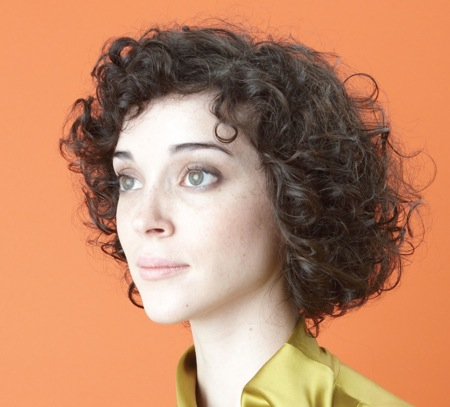
\includegraphics[width=\textwidth]{images/introduction/skin_det_ori3.jpg}
         \caption{}
         \label{fig:skin-detection-ori}
     \end{subfigure}
     \hfill
     \begin{subfigure}[b]{0.45\textwidth}
         \centering
         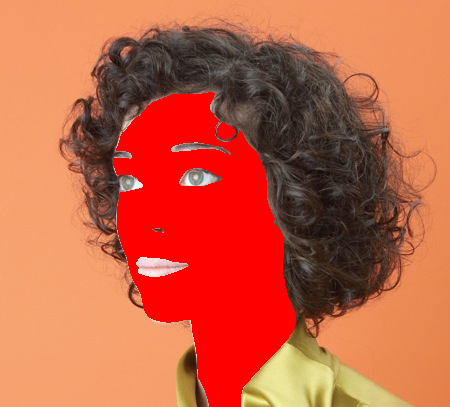
\includegraphics[width=\textwidth]{images/introduction/skin_det_red3.png}
         \caption{}
         \label{fig:skin-detection-red}
     \end{subfigure}
        \caption{Skin detection: (a) original image; (b) detected skin pixels. The original image is part of the Pratheepan dataset~\cite{tan2011fusion}.}
        \label{fig:skin-detection}
\end{figure}

\begin{figure}[h]
     \centering
     \begin{subfigure}[b]{0.3\textwidth}
         \centering
         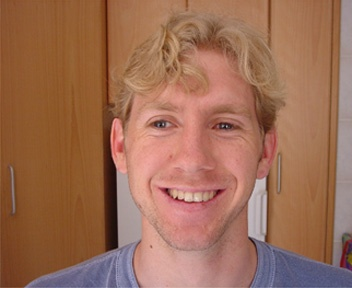
\includegraphics[width=\textwidth]{images/introduction/im00060x.jpg}
         \label{fig:thresh-wood-x}
     \end{subfigure}
     \hfill
     \begin{subfigure}[b]{0.3\textwidth}
         \centering
         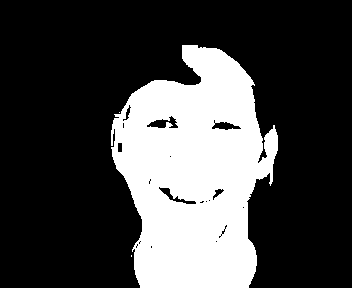
\includegraphics[width=\textwidth]{images/introduction/im00060y.png}
         \label{fig:thresh-wood-y}
     \end{subfigure}
    \hfill
     \begin{subfigure}[b]{0.3\textwidth}
         \centering
         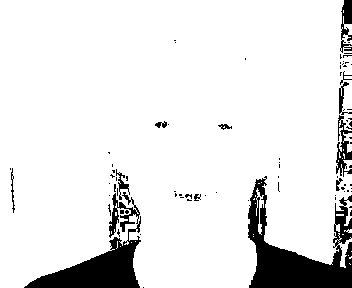
\includegraphics[width=\textwidth]{images/introduction/im00060p.png}
         \label{fig:thresh-wood-p}
     \end{subfigure}
     \begin{subfigure}[b]{0.3\textwidth}
         \centering
         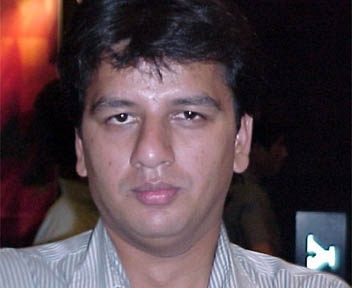
\includegraphics[width=\textwidth]{images/introduction/im00081x.jpg}
         \caption{}
         \label{fig:thresh-color-x}
     \end{subfigure}
     \hfill
     \begin{subfigure}[b]{0.3\textwidth}
         \centering
         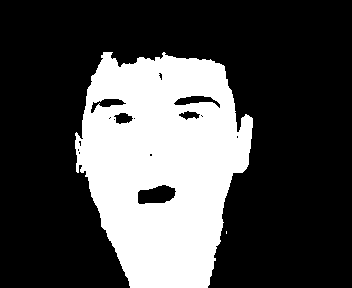
\includegraphics[width=\textwidth]{images/introduction/im00081y.png}
         \caption{}
         \label{fig:thresh-color-y}
     \end{subfigure}
     \hfill
     \begin{subfigure}[b]{0.3\textwidth}
         \centering
         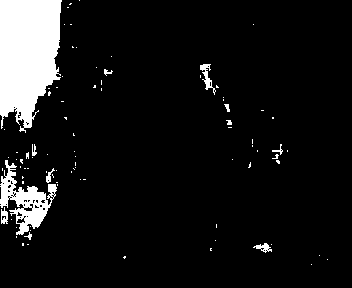
\includegraphics[width=\textwidth]{images/introduction/im00081p.png}
         \caption{}
         \label{fig:thresh-color-p}
     \end{subfigure}
        \caption{Challenges of skin detection, visualized through: (a) the input image, (b) the ground truth, (c) the prediction obtained from a thresholding method~\cite{brancati2017human}.
        The first row depicts an image containing materials with skin-like colors. The second row shows how the colors of an image can be affected by the illumination conditions.}
        \label{fig:common-issues}
\end{figure}

This thesis presents a review of the skin detection datasets and state-of-the-art approaches.
Image databases and state-of-the-art approaches are retrieved, and a new taxonomy is proposed.
Three different computational approaches are selected, thoroughly analyzed, and implemented to compare their strength, weaknesses, generalization capability, and performance.
Before assessing the methods, a validation phase takes place; then the methods are evaluated in single and cross dataset settings over three datasets and three skin tones sub-datasets, using multiple metrics.
Finally, inference times are compared.

The main contributions of this work are the following:
\begin{itemize}
  \item A comparative review of common datasets used in skin detection and discussion on some major data limitations.
  \item An analysis of the state-of-the-art approaches at skin detection, with the proposal for a new taxonomy.
  \item An analysis of some of the evaluation metrics used in binary classification problems.
  \item An in-depth analysis of the three representative state-of-the-art approaches.
  \item An evaluation of the selected approaches on three public datasets in single-dataset and cross-dataset settings.
  \item An evaluation of the selected approaches on three skin tones sub-datasets in single-dataset and cross-dataset settings.
  \item An evaluation of the inferences times of the selected approaches.
\end{itemize}
The thesis is organized as follows: the Chapter \ref{chap:datasets} gives an overview of the datasets used in skin detection including a discussion on the limitations and a detailed description of the three chosen datasets.
Chapter \ref{chap:methods} contains an in-depth analysis of the selected approaches, describing the architecture, functioning, and operations performed by each method.
Chapter \ref{chap:results} contains a detailed explanation of the experiments setup and the evaluation process.
Then, the evaluation results are presented and extensively commented.
Finally, Chapter \ref{chap:conclusion} draws conclusions and gives an outlook on possible future work.

%%%%%%%%%%%%%%%%%%%%%%%%%%%%%%%%%%%%%%%%%%%%%%%%%%%%%%%%%%%%%%%%%%%%%%%%
\section{State of the art}\label{sec:state-of-the-art}
%%%%%%%%%%%%%%%%%%%%%%%%%%%%%%%%%%%%%%%%%%%%%%%%%%%%%%%%%%%%%%%%%%%%%%%%

From a classification point of view, skin-color detection can be seen as a two-class problem: skin-pixel vs. non-skin-pixel classification. The problem has been approached in different ways, which aren't uniquely categorizable.
Researchers have categorized the methods mainly in two groups: segmentation-based~\cite{naji2019survey} and classification-based~\cite{brancati2017human}. With the advent of deep learning, the former categorization becomes more ambiguous. In fact, Machine Learning methods include both approaches based on the analysis of individual pixels, such as traditional methods, and approaches that use the pixel neighbors information, such as CNNs.\\
A new classification-based taxonomy based is proposed, \autoref{fig:taxonomy}. It categorizes skin detector methods into the following groups: rule-based, machine learning and hybrid.\\
\textbf{Rule-based} methods use plain rules to classify each pixel as either skin or non-skin. Thresholding and fuzzy logic systems are part of this group.\\
\textbf{Machine learning} approaches construct models from a training set of data to use in classification.
They describe a broad range of techniques, which can be subdivided into statistical, deep learning and ensemble categories.\\
\textbf{Hybrid} approaches make use of a cluster of different techniques working together to perform the classification. A common choice is to stack a region-based algorithm on top of the result of other classification methodologies. \\

\begin{figure}[h]
	\centering
	
\includegraphics[width=0.9\linewidth]{images/introduction/taxonomy.png}
	\caption{Taxonomy of skin detectors.}
	\label{fig:taxonomy}
\end{figure}

\noindent{This section describes some common skin detection approaches. A chronological organization of the review with regards to the proposed taxonomy is reported in \autoref{tab:state-of-the-art}.}\\
\textbf{Jones and Rehg 2002}~\cite{jones2002statistical} is a machine learning statistical method based on the construction of a skin-color histogram model from an image database.
Then, a Bayesian classifier uses the model to make predictions on the desired images. The histogram model is built from an image database by analyzing the frequency that every pixel (R,G,B) combination has to be either skin or non-skin.
The Bayes rule utilizes a threshold to classify pixels based on their probability of being skin pixels.\\
\textbf{Kovac \textit{et al.} 2003}~\cite{kovac2003human} is a rule-based thresholding method that uses the union of a pair of rules to segment skin regions.
The first rule specializes in finding skin at uniform daylight illumination.
The second rule specializes in finding skin under flashlight or lateral daylight illumination.\\
\textbf{Chen and Wang 2007}~\cite{chen2007region} is a hybrid approach consisting of four main stages: image segmentation, key skin region extraction, similarity measurement, and skin region classification.
In the first stage, an unsupervised segmentation of color-texture regions in images is applied to segment the image into homogeneous regions.
In the second stage, a skin extractor is used for extracting the key skin regions. Firstly, the candidates of key skin regions are chosen by a rule-based skin classifier.
Then, the confidence values of the candidate regions are calculated as the proportion of the detected skin pixel count to the total pixel count of the region. The region with the largest confidence value will be the key skin region.
In the third stage, the similarity measure between the key skin region and all other regions is calculated to merge more possibly skin regions.
In the last stage, an algorithm is used to determine whether a region should be classified as a skin region or a non-skin region.
The algorithm calculates the pixels overlap ratio of the two 2D skin-color histograms representing a region and the key skin region, and then utilizes a threshold to classify the region.\\
\textbf{Khan \textit{et al.} 2010}~\cite{khan2010skin} is a machine learning ensemble approach that utilizes a random forest, an ensemble of tree predictors, to classify skin regions.
The input is presented to each of the trees in the forest.
Each tree gives an independent classification prediction and \q{votes} for that class.
The forest chooses the classification having the most votes. An image database is used to train the forest trees.\\
\textbf{Iraji and Yavari 2011}~\cite{iraji2011skin} is a rule-based fuzzy logic approach that defines a set of rules in the YCbCr color space to distinguish skin and non-skin pixels.
There may be pixels whose color acts both as skin color and as non-skin color.
Thanks to fuzzy logic with a Mamdani inference system (based on the implication rules), it is possible to get a unique membership value for each pixel, making the classification straightforward.\\
\textbf{Kawulok \textit{et al.} 2014}~\cite{Kawulok2014EURASIP} is a hybrid method that combines spatial analysis on top of a machine learning classifier.
First, the input image is converted into a skin probability map using a statistical histogram skin color model and a Bayesian classifier.
Then, the probability map is processed to find seed pixels.
The initial seed pixels are expanded using distance transform to include more skin pixels.
Subsequently, a local skin color model is trained from the obtained result and used to detect further skin pixels.
Finally, the distance transform is applied one more time.\\
\textbf{Brancati \textit{et al.} 2017}~\cite{brancati2017human} is a rule-based thresholding approach that works in the YCbCr color space.
Dynamic correlation rules are used to evaluate the combinations of chrominance values to identify the skin pixels in the YCb and YCr subspaces.
The correlation rules depend on the shape and size of dynamically generated skin color clusters computed in the YCb and YCr subspaces.\\
\textbf{He \textit{et al.} 2019}~\cite{he2019semi} is a deep learning method based on a dual-task CNN for joint detection of skin and body.
The dual-task network contains a shared encoder but two decoders for skin and body separately.
For each decoder, its output also serves as a guide for its counterpart, making both decoders mutually guided.\\
\textbf{Tarasiewicz \textit{et al.} 2020}~\cite{tarasiewicz2020skinny} proposed Skinny, a deep learning approach based on an encoder-decoder CNN architecture called U-Net.
Inception and dense block are inserted into a modified U-Net architecture to benefit from a wider spatial context.\\

\begin{table}[!htbp]
    \centering
    \resizebox{\textwidth}{!}{
    \begin{tabular}{lccc}
    \toprule
    \textbf{Name} & \textbf{Year} & \textbf{Category} & \textbf{Subcategory} \\
    \midrule
         Tarasiewicz \textit{et al.}~\cite{tarasiewicz2020skinny} & 2020 & Machine Learning & Deep Learning: CNN\\
         He \textit{et al.}~\cite{he2019semi} & 2019 & Machine Learning & Deep Learning: CNN\\ % Dual Decoder
         Brancati \textit{et al.}~\cite{brancati2017human} & 2017 & Rule-based & Thresholding\\
         Kawulok \textit{et al.}~\cite{Kawulok2014EURASIP} & 2014 & Hybrid & Machine Learning + Spatial Analysis\\ % Spatial Analysis
         Iraji and Yavari~\cite{iraji2011skin} & 2011 & Rule-based & Fuzzy Logic\\
         Khan \textit{et al.}~\cite{khan2010skin} & 2010 & Machine Learning & Ensemble: RandomForest\\
         Chen and Wang~\cite{chen2007region} & 2007 & Hybrid & Rule-based + Region-growing\\
         Kovac \textit{et al.}~\cite{kovac2003human} & 2003 & Rule-based & Thresholding\\
         Jones and Rehg~\cite{jones2002statistical} & 2002 & Machine Learning & Statistical: Bayes\\
    \bottomrule
    \end{tabular}}
  \caption{%
    Common approaches to Skin Detection, sorted by year in descending order.
  }
  \label{tab:state-of-the-art}
\end{table}
